\subsection{Introducción}\label{header-n2}

Partiendo por la definición del caso anterior, se realizan cambios en la
geometría para adecuar el modelo a un estudio en 3-D. Entre las
herramientas descritas en el apartado {[}XXDescripción de
herramientas{]} se experimenta con \emph{snappyHexMEsh}, \emph{cfMesh} y
\emph{Salome}. Las tres ofrecen mallados automatizados, los dos primeros
están escritos en el mismo lenguaje que OpenFOAM, en cambio el tercer
software se asemeja a un programa de CAD, dispone de interfaz gráfica e
implementa diferentes algoritmos para realizar el mallado.

En un primer lugar, se trató de alcanzar la solución con los dos
primeros, dado que por el lenguaje en el que están escritos los archivos
ocupan menos, una vez definidos tardan menos en procesar la solución y
consumen menos memoria. No obstante, resulta más complicado detectar los
errores que se producen. Por ello, a pesar de que se hubieran ejecutado
exitósamente para casos más sencillos, finalmente se genera a partir de
\emph{Salome}.

La geometría del caso final se obtiene una vez alcanzado el modelo de
ensayo deseado, tomando las medidas lo más exactas posibles a la
disposición real del ensayo. A parte de esto, se realizan diferentes
pruebas variando el diámetro del diafragma
\textbf{{[}8-9,5-11-12,5-14-15,5-16{]}mm}.

Sin embargo, dado que el aparato de medida de la presión que se va a
utiliza en el laboratorio está limitado a 100Pa, para preservar su
funcionamiento se ensayarán los diafragmas que no sobrepasen dicha
medición. A partir de los resultados que a continuación se describen,
para el diafragma de diámetro 12,5 mm se obtiene una presión por encima
de 120Pa. Por ello, se añade el caso para un diafragma de diámetro
\textbf{13 mm}, y así disponer de cuatro pruebas diferentes para
comparar con el experimento.

La estructura del caso, que se mantiene del problema anterior realizado
en 2-D, es la siguiente:

\begin{verbatim}
+ <case>
-+ 0
--- alpha.water
--- alpha.water.orig
--- epsilon
--- k
--- nut
--- nuTilda
--- p_rgh
--- U
-+ constant
--- g
--- transporProperties
--- turbulenceProperties
-+ system
--- setFields
--- fvSchemes
--- fvSolution
--- controlDict
\end{verbatim}

A esta se le añade el modelo generado a partir de Salome y convertido a
formato OpenFOAM a través de una orden por terminal, detallada en
\href{https://cfd.direct/openfoam/user-guide/mesh-conversion/}{User
Guide: 5.5 Mesh conversion}; así como, los ficheros necesarios para
extraer los resultados.

\subsection{Definición del caso}\label{header-n18}

\begin{figure}
\centering
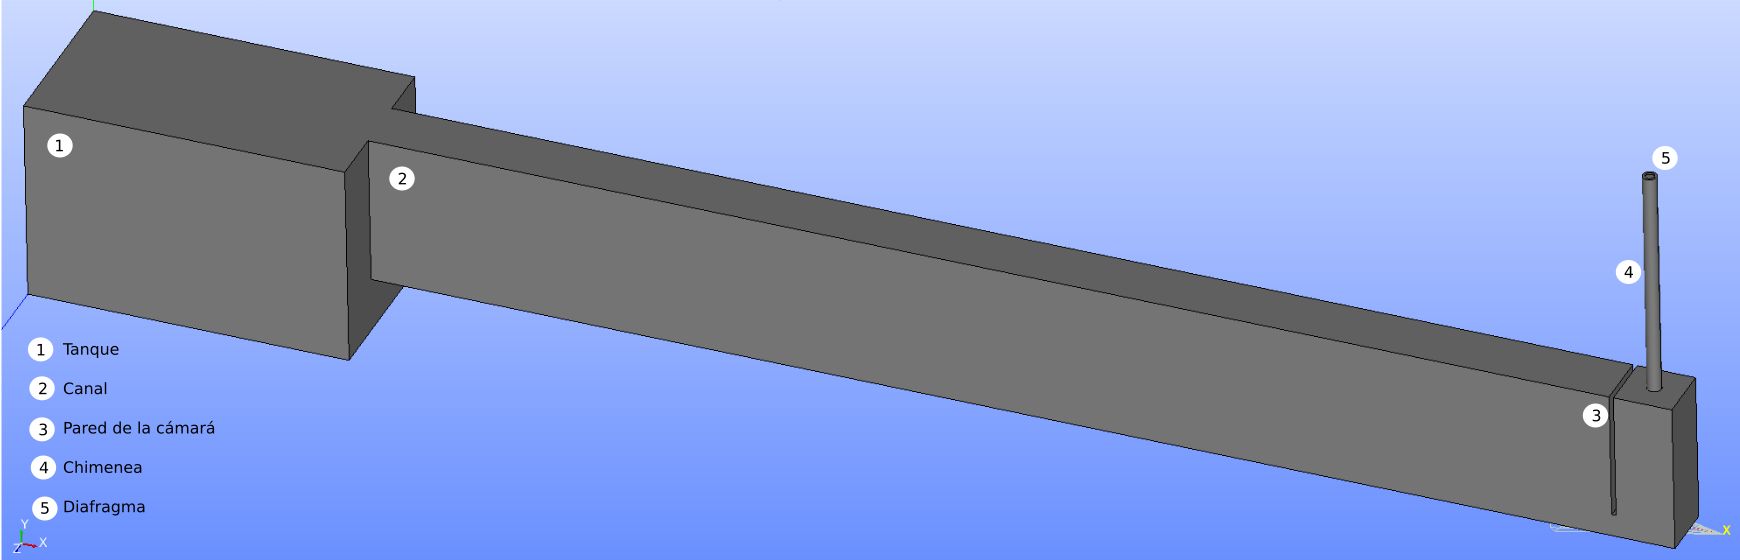
\includegraphics{geomCanal3D.png}
\caption{Representación del modelo del caso}
\label{fig:geomCanal3D}
\end{figure}

\begin{figure}
\centering
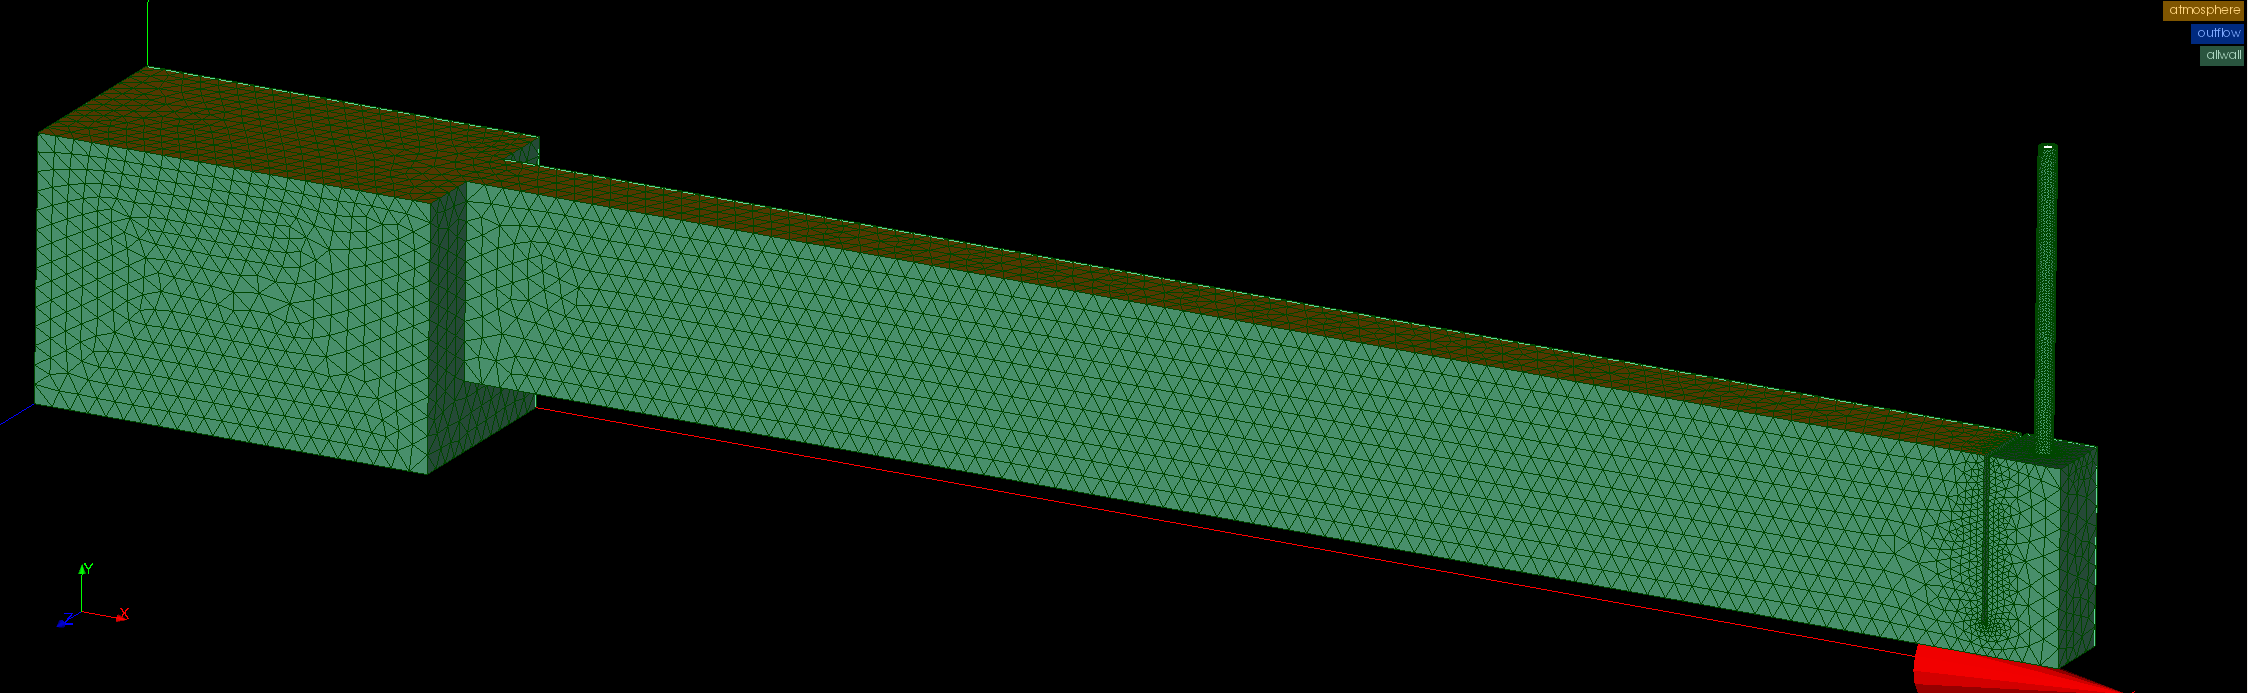
\includegraphics{D13bdry.png}
\caption{Mallado y contornos del modelo (\emph{atmosphere, allwall, outflow})}
\label{fig:D13bdry}
\end{figure}

\begin{itemize}
\item
  Objetivos del caso:

  \begin{itemize}
  \item
    Obtener una solución que se aproxime lo máximo posible al ensayo
    real que se realizará en el laboratorio.
  \item
    Hallar la altura del agua dentro de la cámara; la presión
    manométrica aguas arriba del diafragma; y el caudal a través del
    diafragma. A partir de estos valores, se define la potencia para
    cada diafragma, como una forma equivalente de representar lo que
    resultaría colocando una turbina.
  \end{itemize}
\item
  Generación del modelo a partir de \emph{Salome}:

  \begin{enumerate}
  \def\labelenumi{\arabic{enumi}.}
  \item
    Para comenzar, se genera un modelo que sirva de base para realizar
    las diferentes pruebas variando el diámetro del diafragma. Aunque se
    permita importar un modelo en STL, como se tienen superficies
    curvas, el número de fragmentos en los que se descomponen estas
    superficies es demasiado alta para asociarlas a una misma región o
    contorno. Por ello, se guarda la geometría , generada desde la misma
    herramienta, hasta la definición del diafragma. A continuación se
    representan las medidas (en metros) de los objetos definidos:

    \begin{itemize}
    \item
      Tanque: (0.44 0.285 0.236).
    \item
      Canal: (1.786 0.21 0.08), con una translación de (0.44 0.075
      0.078).
    \item
      Pared de la cámara: (.006 .178 .08), con una translación de (2.14
      0.107 0.078).
    \item
      Chimenea: (R=0.0098 H=0.321), con una rotación de (90 0 0) y
      revertido 90º respecto del eje 'x'; y una translación de (2.186
      0.285 0.118).
    \end{itemize}
  \item
    A partir de aquí, se repeten los pasos para cada diafragma, tomando
    como ejemplo el de diámetro \textbf{13mm}. Por un lado, se termina
    la geometría del modelo con la definición del diafragma y, por otro,
    se realizan las operaciones de cortes y uniones necesarias:

    \begin{itemize}
    \item
      Diafragma: (R=0.0065 H=0.002), con una rotación de (-90 0 0); y
      una translación de (2.186 .604 0.118).
    \end{itemize}

    Operaciones booleanas:

    \begin{itemize}
    \item
      Corte para definir la pared de la cámara: Cut (Main object- canal;
      Tool Object-\textgreater{} chamber wall).
    \item
      Corte para implementar el diafragma: Cut (Main
      object-\textgreater{} chimney; Tool Object-\textgreater{} diaf).
    \item
      Unión: Fuse (Tank, cut1, cut2).
    \end{itemize}

    Dando como resultado la siguiente imagen:

    \autoref{fig:geomCanal3D}

  \item
    Definición de contornos:

    En este caso, la definición de los contornos que conformarán el
    modelo, también se definen desde la propia herramienta:

    \begin{itemize}
    \item
      Primero se obtienen las caras del modelo, mediante la opción
      \texttt{Explode}.
    \item
      Después, se crean los grupos de caras, que conformarán cada
      contorno (\emph{atmosphere, outflow, allwall}) desde el menú
      seleccionando \texttt{Create\ new\ Group}. Se aconseja guardar
      tras este paso .
    \end{itemize}
  \item
    Generación de la malla:

    Se analizan diferentes alternativas para el mallado, implementadas
    en la herramienta. De entre ellas, como el dominio tiene partes
    curvas, la descomposición más sencilla, resulta la tetraédrica, la
    cual se realiza mediante el algoritmo \emph{Netgen}. Accediendo
    desde el menú a la opción \texttt{Create\ Mesh}, se define con los
    siguientes parámetros:

    \begin{itemize}
    \item
      Tipo de malla: Tetraédrica.
    \item
      Algoritmo: Netgen 1D-2D-3D.
    \item
      Hipótesis: Netgen 3D Parameters; con unas dimensiones de las
      celdas Max=0.020 y Min =0.002; y un refinado fino.
    \end{itemize}

    Tras computar la malla para el caso de ejemplo, el número de celdas
    es de: \textbf{90710 tetraedros}.
  \item
    Exportar la malla junto con los contornos:

    Antes de exportar la malla, será necesario reconocer los contornos
    antes definidos, con la creación de grupos de malla desde la
    geometría, tal y como se explica en el tutorial
    \href{http://staff.um.edu.mt/__data/assets/pdf_file/0016/106144/Salome_to_OpenFOAM.pdf}{Salome
    to OpenFOAM mesh conversion tutorial}.

    Entonces, para definir estos contornos sobre la malla creada, se
    selecciona desde el menú, la opción
    \texttt{Create\ Groups\ from\ Geometry} y se especifica el grupo de
    caras correspondiente a cada contorno, el resultado final se puede
    apreciar en la siguiente imagen:\\

    \autoref{fig:D13bdry}

    Una vez hecho esto, en el árbol de objetos se puede observar que
    dentro de la malla definida, se encuentran los contornos generados.
    Finalmente, se exporta la malla, junto con los contornos, a formato
    UNV, el cual es compatible con OpenFOAM.
  \item
    Se añade al caso el modelo exportado a UNV y se convierte a formato
    de OpenFOAM mediante la siguiente orden por terminal:

\begin{verbatim}
ideasUnvToFoam filename.unv
//transformPoints -scale '(0.001 0.001 0.001)'//change from mm to m
\end{verbatim}

    Tras este paso, hay que modificar manualmente la característica de
    la pared desde
    \textless{}./constant/polyMesh/boundary\textgreater{}, para la
    región \emph{allwall}: \texttt{patch\ -\textgreater{}\ wall}.
  \end{enumerate}
\item
  Condiciones iniciales:

  La condición inicial del agua, descrita en
  \textless{}./system/setFieldsDict\textgreater{}, se establece mediante
  la diagonal definida por dos puntos, los cuales constituirán el
  rectángulo, cuyas celdas contendrán agua:

  \begin{itemize}
  \item
    Rectángulo 1: (0 0 -1) (0.6 0.22 1)
  \item
    Rectángulo 2: (0.6 0 -1) (2.226 0.12 1)
  \end{itemize}

  Las dimensiones no importa que sobrepasen las medidas del dominio, ya
  que sólo se describirán con agua las celdas que se encuentren sobre el
  modelo y no resultará en errores.
\end{itemize}

\begin{figure}
\centering
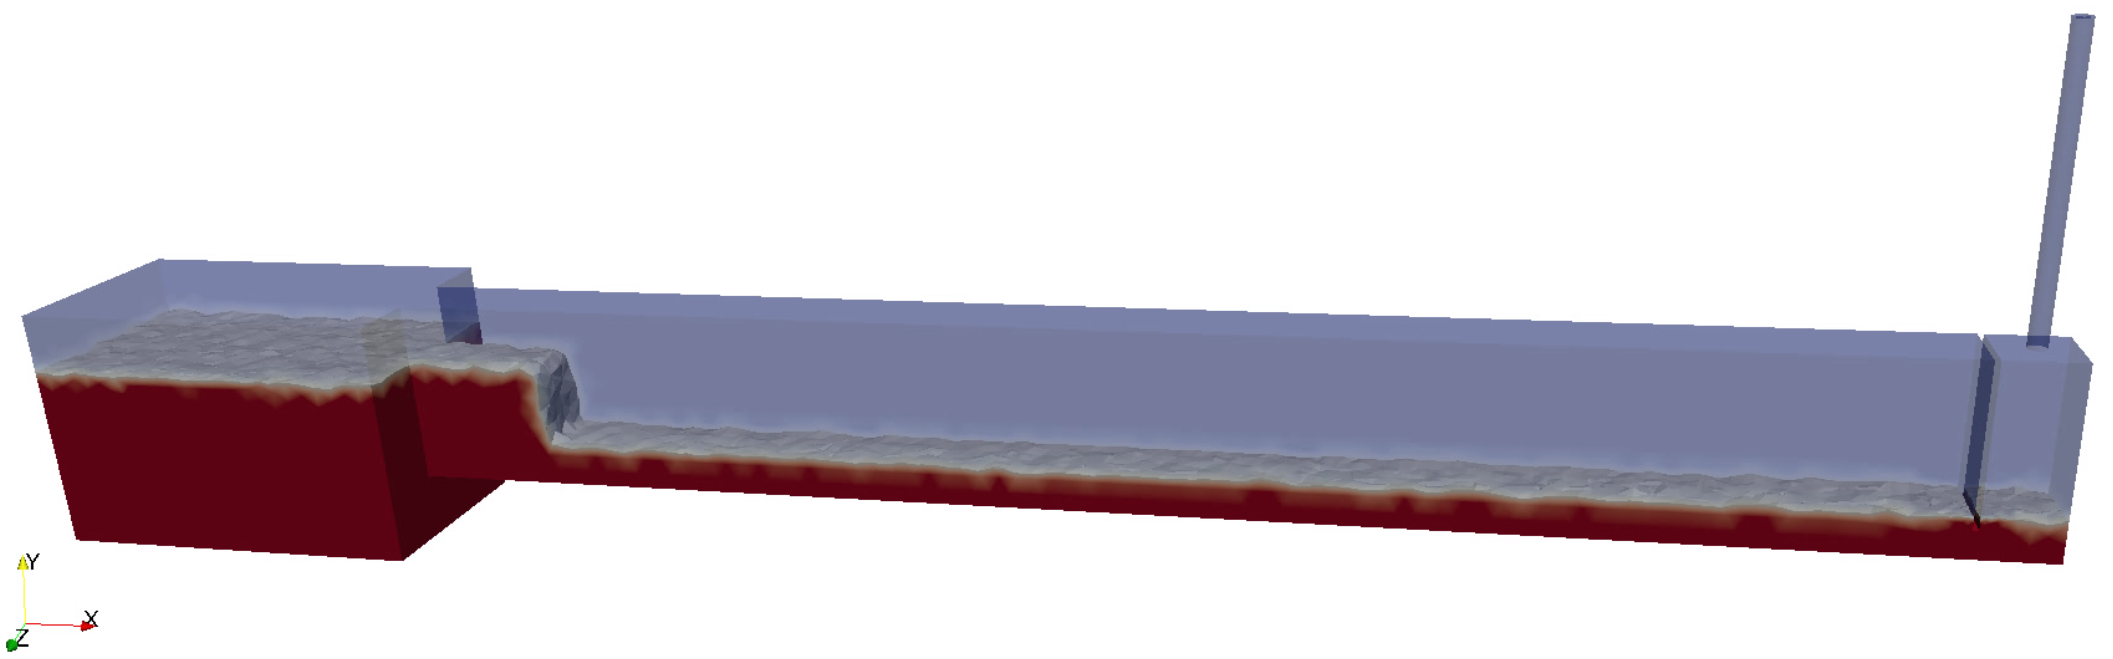
\includegraphics{D12wl.png}
\caption{Representación del problema en el instante inicial}
\label{fig:D12wl}
\end{figure}

\subsection{Ejecución}\label{header-n149}

La ejecución de este caso se puede realizar mediante el \emph{script} ,
o bien con si se ejecuta desde \emph{Docker} con Windows 10. Las
instrucciones descritas en los mismos, corresponden a lo siguiente:

\begin{enumerate}
\def\labelenumi{\arabic{enumi}.}
\item
  Comprobar si la malla antes creada es correcta:

\begin{verbatim}
checkMesh | tee log.checkMesh
\end{verbatim}
\item
  Definir la condición inicial del volumen ocupado por agua con la
  orden:

\begin{verbatim}
 setFields > log.setFields
\end{verbatim}
\item
  Procesar el caso con la orden:

\begin{verbatim}
interFoam > log.interFoam &
\end{verbatim}

  La entrada \texttt{\&} ejecuta el proceso en segundo plano, de esta
  forma se pueden monitorizar los residuos en tiempo real, con las
  librerías y \emph{scripts} necesarios escritos en \emph{Python}, ver
  \href{https://openfoamwiki.net/index.php/Contrib/PyFoam\#Runner-Utilities}{Contrib/PyFoam}:

\begin{verbatim}
pyFoamPlotWatcher.py log.interFoam
\end{verbatim}
\end{enumerate}

\begin{figure}
\centering
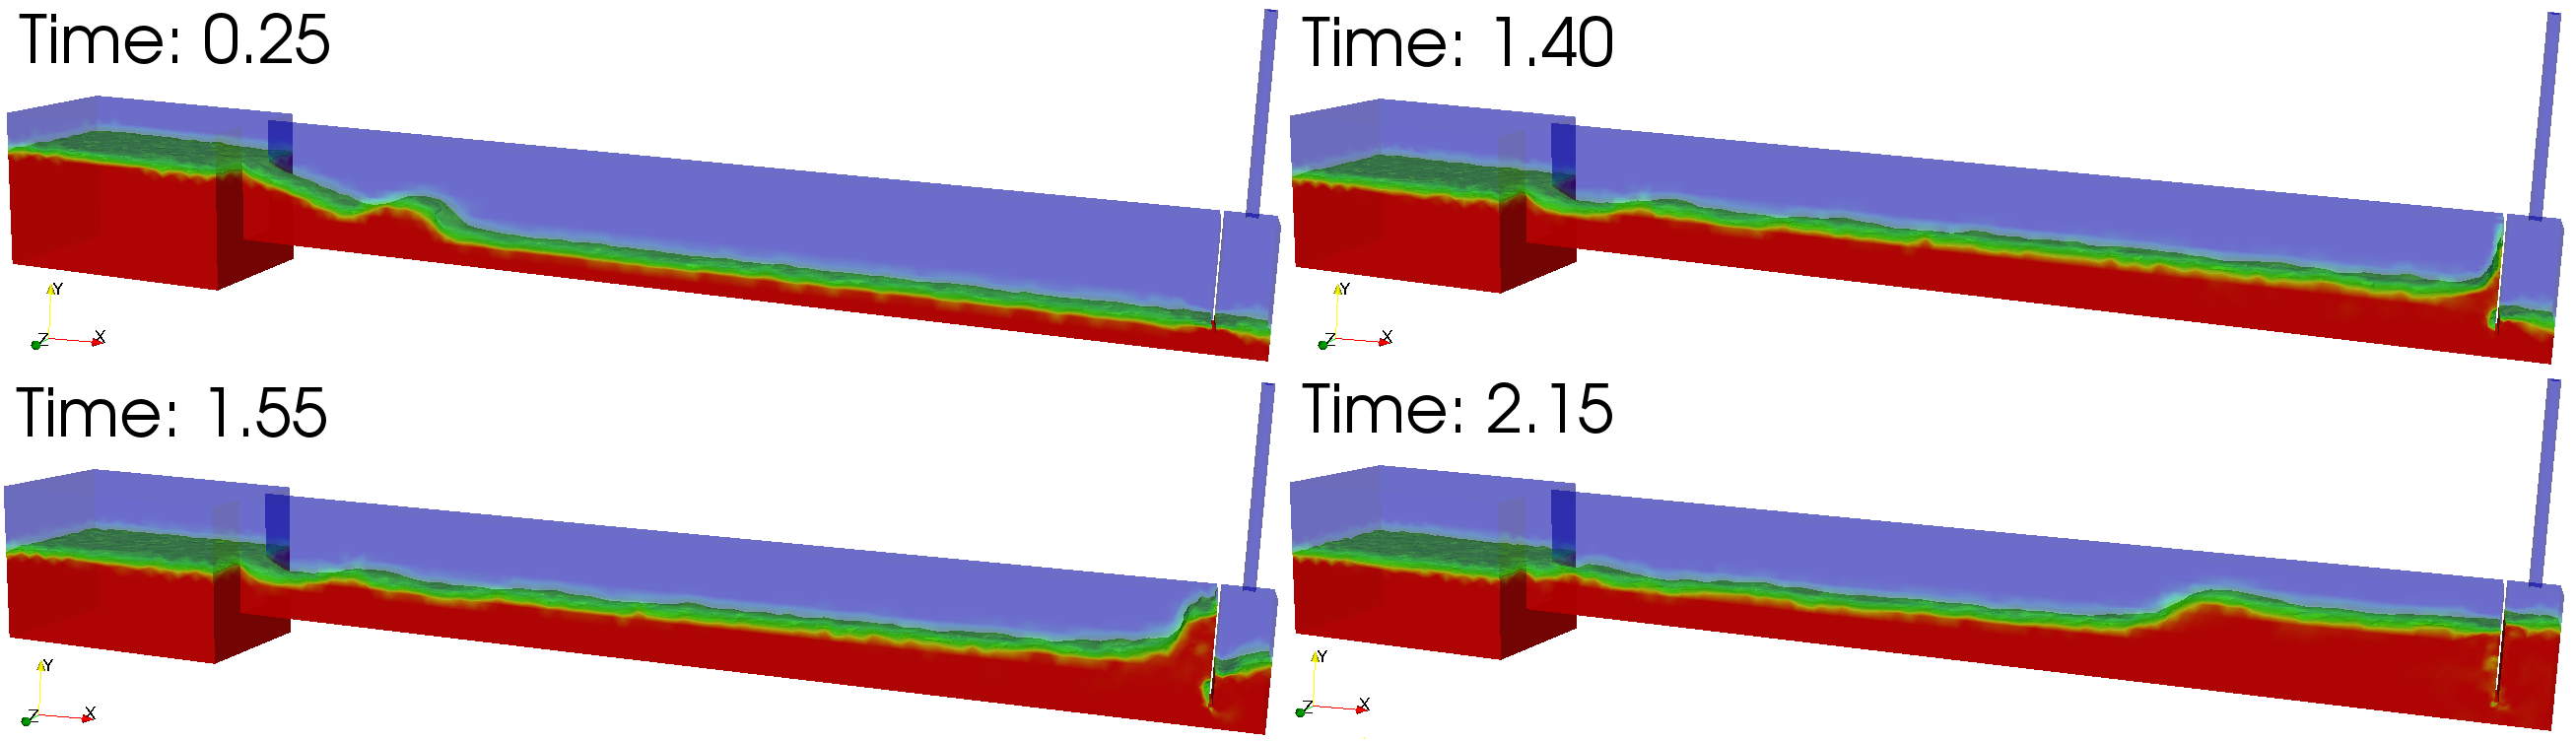
\includegraphics{D13canal3D.png}
\caption[Visualización del caso 3D]{Visualización del caso 3D, con la representación de la fracción de agua}
\label{fig:D13canal3D}
\end{figure}

\subsection{Resultados}\label{header-n176}

De forma análoga al caso en 2-D, el flujo de salida a través del
diafragma se obtiene mediante la función \emph{outletFlux}, definida en
\textless{}./system/controlDict\textgreater{}, durante la simulación. La
altura y la presión se hallan desde \emph{ParaView} ejecutando un
\emph{script} de \emph{Python}; y a partir de estos valores se consiguen
diferentes formas de representar la solución por medio de \emph{Octave}.

Por tanto, se añaden al caso los siguientes ficheros para la obtención
de los resultados tras el procesado de la solución:

\begin{verbatim}
-- prgh.py
-- water_level.py
-- WL.m
-- Prgh.m
-- QT.m
-- potT.m
-- HQ.m
\end{verbatim}

\begin{figure}
\centering
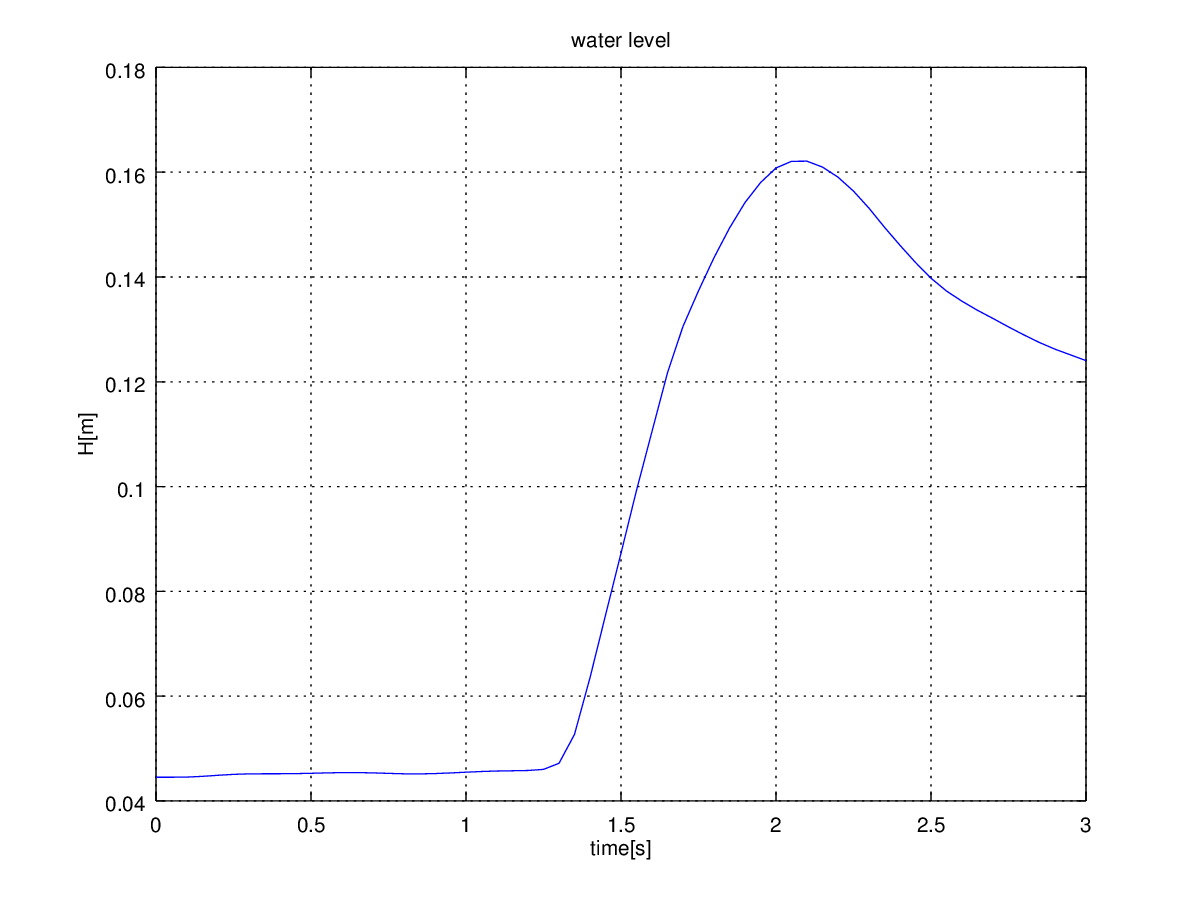
\includegraphics{wlCanal3D.png}
\caption{Altura del nivel del agua dentro de la cámara}
\label{fig:wlCanal3D}
\end{figure}

\begin{enumerate}
\def\labelenumi{\arabic{enumi}.}
\item
  Altura del nivel del agua dentro de la cámara:

  Descrito en el caso en 2-D, este resultado se obtiene ejecutando el
  \emph{script} \textless{}./water\_level.py\textgreater{} desde el menú
  de \emph{ParaView} (Tools\textgreater{}Python Shell), el cual guarda
  los resultados en la carpeta del caso
  \textless{}./waterlevel.csv\textgreater{} y se grafica mediante un
  \emph{script} realizado desde \emph{Octave}.

  Debido a que las operaciones necesarias (p.e. la integración de los
  valores de la altura del agua para hallar la media) se realizan en el
  \emph{script} de \emph{Python}, las instrucciones desde Octave, se
  resumen en: definir una matriz que contenga la tabla de valores,
  siendo el vector 'x' el tiempo y el 'y' la altura, y graficar
  directamente estos datos.

  \autoref{fig:wlCanal3D}

\item
  Caudal de salida:

  La función definida en el diccionario
  \textless{}./system/controlDict\textgreater{} es la siguiente:

\begin{verbatim}
functions
{
 outletFlux
    {
        type            surfaceRegion;
        libs ("libfieldFunctionObjects.so");
        writeControl   timeStep;
        log             true;
        // Output field values as well
        writeFields     false;
        regionType      patch;
        name            outflow;
        operation       sum;

        fields
        (
            rhoPhi
        );
    }
\end{verbatim}

  A lo largo de la simulación, esta función calcula el valor de
  \(\text rhoPhi=\frac {kg}{m^3} \frac {m}{s}= \frac {kg}{s} · \frac {1}{m^2}\),
  es decir, el caudal másico por unidad de área, y se guarda en
  \textless{}./postProcessing/outletFlux/0/surfaceRegion.dat\textgreater{}.

  Para obtener la gráfica, se prepara un \emph{script} desde
  \emph{Octave} \textless{}./QT.m\textgreater{}, donde se leen los datos
  (del caudal y del tiempo) y se guardan en una matriz. El valor del
  caudal se da como caudal másico, luego se divide entre
  \(\rho=1,21kg/m^3\) para conseguir la unidad del Sistema Internacional
  (S.I.) {[}\(m^3/s\){]}. Por último, se representan los valores del
  paso del tiempo respecto del caudal.

\end{enumerate}

\begin{figure}
\centering
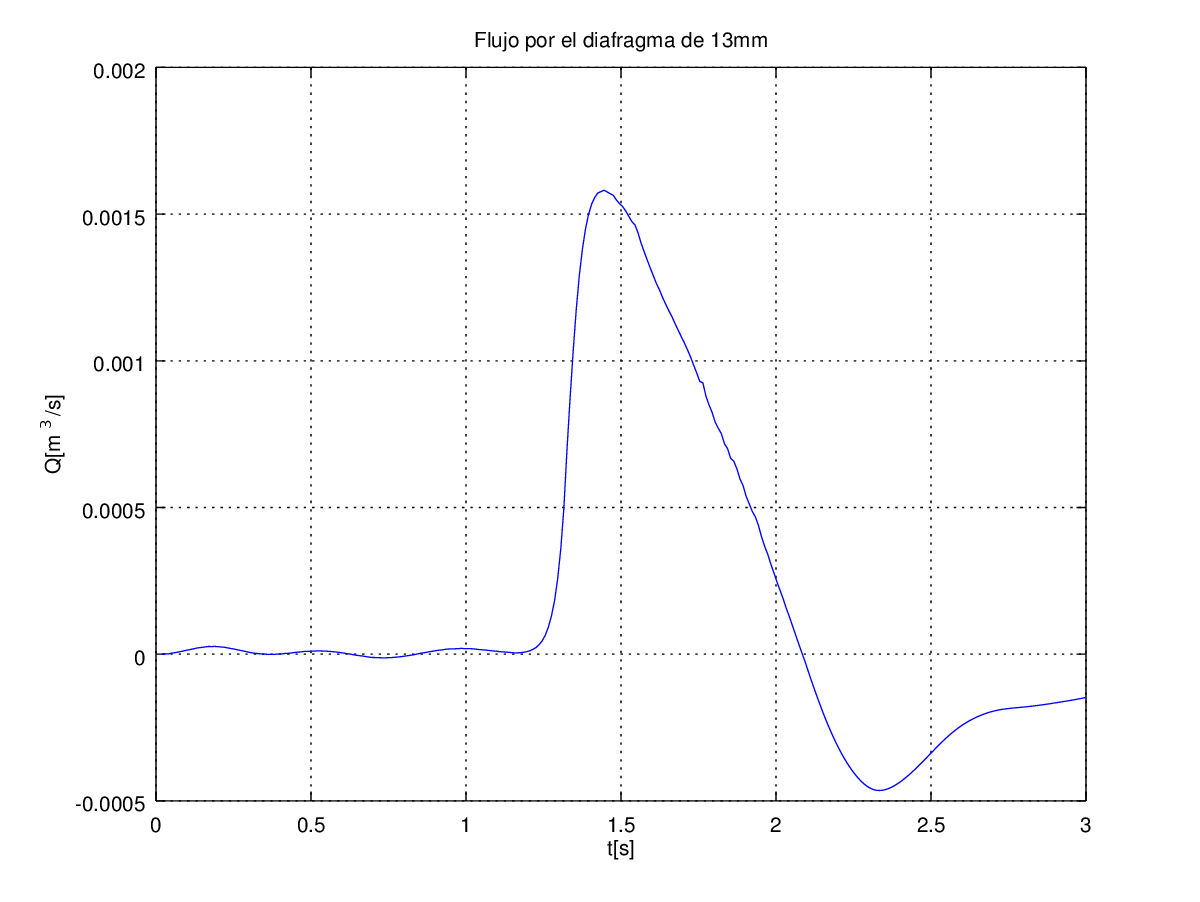
\includegraphics{QTCanal3D.png}
\caption{Caudal a través del diafragma}
\label{fig:QTCanal3D}
\end{figure}

\begin{figure}
\centering
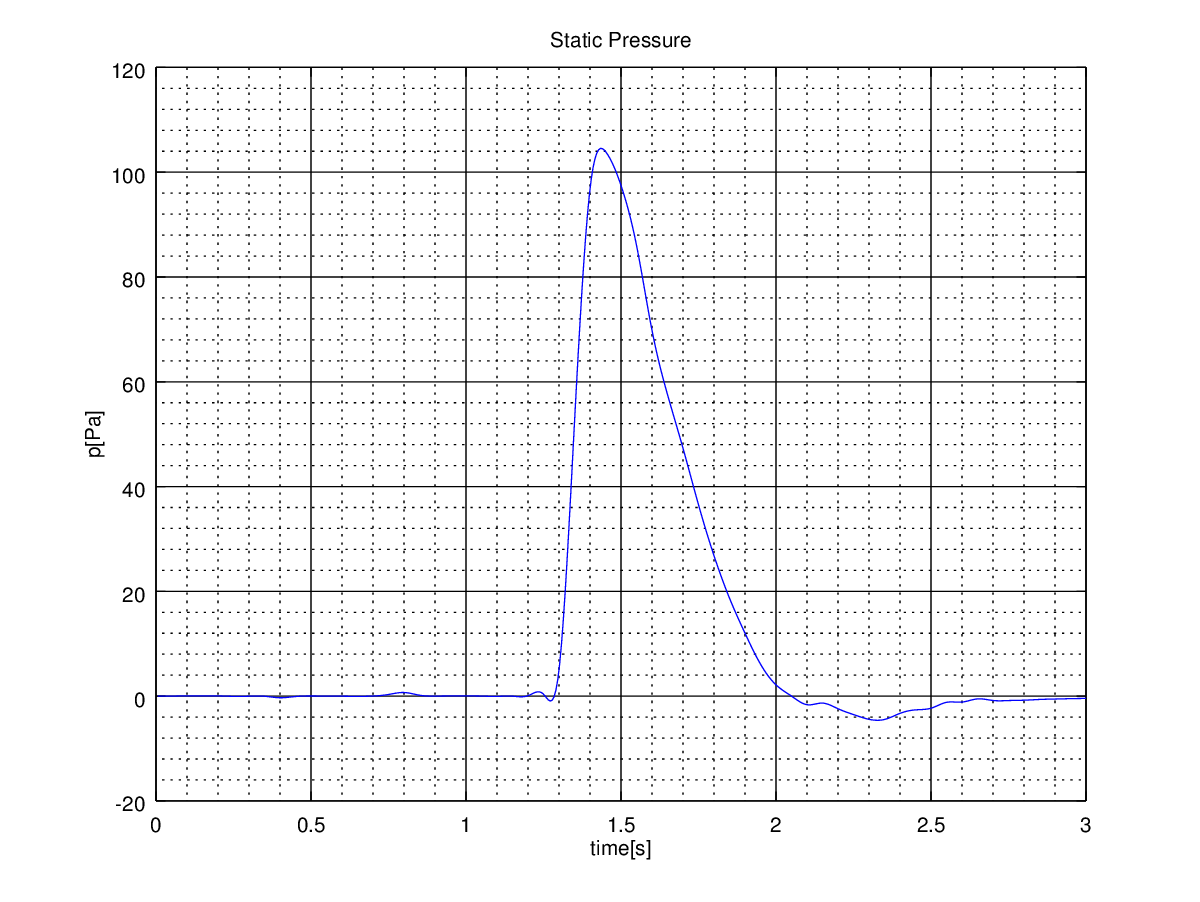
\includegraphics{PmCanal3D.png}
\caption{Presión manométrica en el punto indicado}
\label{fig:PmCanal3D}
\end{figure}

\begin{figure}
\centering
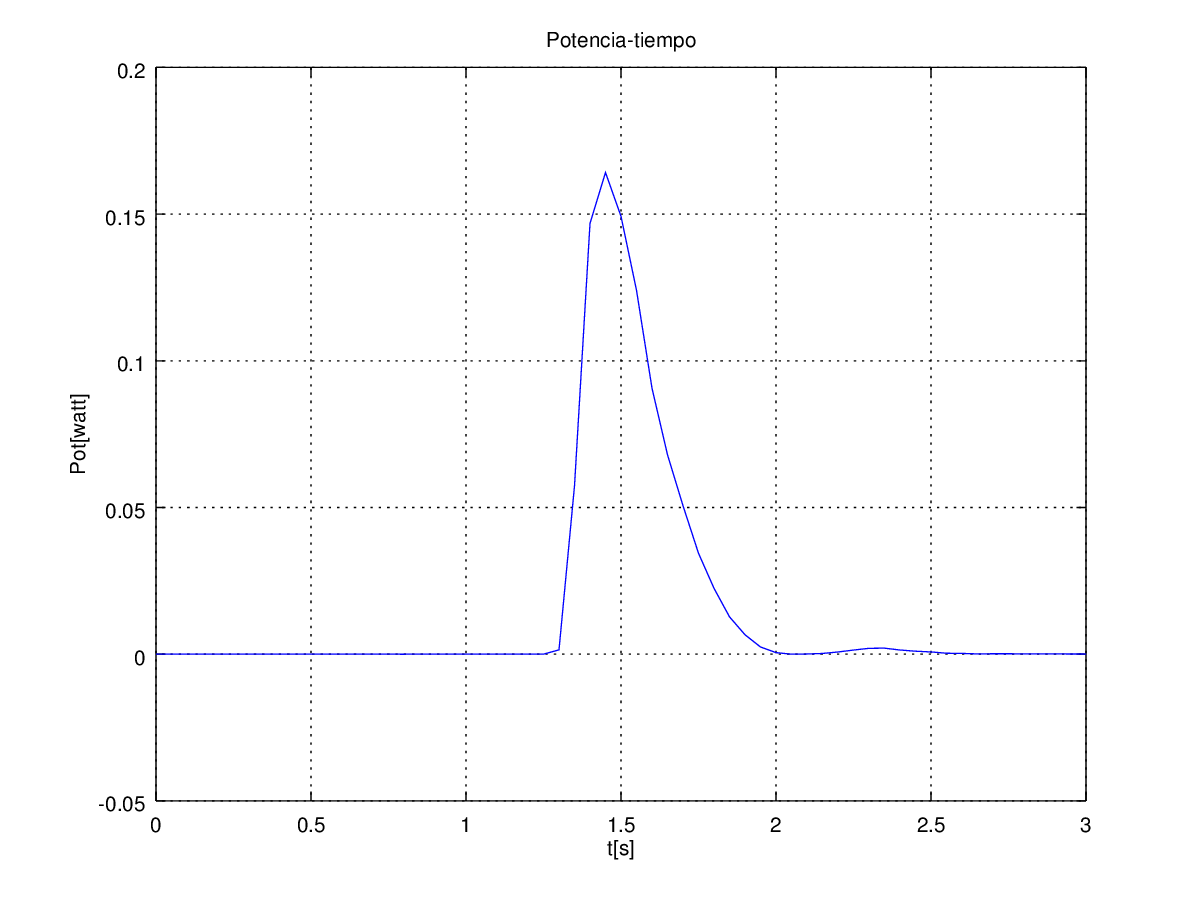
\includegraphics{potTCanal3D.png}
\caption[Potencia máxima]{Potecia equivalente a la diferencia de presiones por el caudal a través del diafragma}
\label{fig:potTCanal3D}
\end{figure}

\begin{enumerate}
\def\labelenumi{\arabic{enumi}.}
\item
  Presión estática:

  La presión manométrica aguas arriba del diafragma, al igual que en el
  caso en 2-D, se logra de forma automatizada mediante el \emph{script}
  \textless{}./prgh.py\textgreater{} ejecutado desde \emph{ParaView}. De
  este fichero se modifican los campos correspondientes a la carpeta del
  caso a la que se debe apuntar y se indica el punto de medición
  correspondiente, detallado en el ensayo, {[}2.186, 0.582, 0.118{]}m.
  Los resultados se guardan en
  \textless{}./rghPressure.csv\textgreater{} donde la variable calculada
  \emph{P\_rgh}, definida en el código de OpenFOAM en , tiene unas
  unidades de {[}\(kg/ms^2\){]} lo que es lo mismo que {[}\emph{Pa}{]}.
  Como en los casos anteriores a partir de \emph{Octave} se grafican.

  \autoref{fig:PmCanal3D}

\begin{enumerate}
\def\labelenumi{\arabic{enumi}.}
\item
  Potencia teórica obtenida:

  La potencia se calcula a partir de la ecuación: \(Pot=\Delta P·Q\),
  como estos valores son conocidos, se utiliza \emph{Octave} para
  automatizar la solución del gráfico en base a los siguientes
  critérios:

  \begin{itemize}
  \item
    El caudal másico se divide entre \(\rho=1,21kg/m^3\) para obtener el
    caudal en {[}\(m^3/s\){]}.
  \item
    El valor de la diferencia de presiones, corresponde a la presión
    manométrica hallada, ya que el segundo punto se sitúa a presión
    atmosférica.
  \item
    La dimensión de la matriz para el caudal, por manera en la que se ha
    obtenido (durante la simulación), tiene más valores intermedios, con
    lo que se reduce a la dimensión de la presión, la cual contiene los
    valores para cada paso del tiempo definido.
  \item
    Finalmente, se multiplican los vectores de ambas columnas (presión y
    caudal) y se grafica respecto del tiempo.
  \end{itemize}

  \autoref{fig:potTCanal3D}

\end{enumerate}

\subsection{Conclusiones}\label{header-n249}

Como se ha mencionado con anterioridad, a partir de los valores hallados
desde \emph{OpenFOAM} y \emph{ParaView}, se obtienen los valores de la
potencia para cada diafragma utilizado. A modo resumen, a continuación
se presenta la solución de cada caso:

\begin{longtable}[]{@{}ccccc@{}}
\caption{Resultados obtenidos para cada modelo}
\toprule
D {[}mm{]} & \(H_{máx}\) {[}m{]} & \(Q_{máx}\) {[}m³/s{]} &
\(\Delta P_{máx}\) {[}Pa{]} & \(Pot_{máx}\) {[}Watt{]}\tabularnewline
\midrule
\endhead
8 & 0,22454 (t=2,3s) & 0,001003 (t=1,4s) & 446,646 (t=1,4s) & 0,44813
(t=1,4s)\tabularnewline
9,5 & 0,22978 (t=2,20s) & 0,001235 (t=1,45s) & 318,92 (t=1,4s) & 0,39346
(t=1,4s)\tabularnewline
11 & 0,23653 (t=2,1s) & 0,0014654 (t=1,45s) & 204,14 (t=1,45s) & 0,29915
(t=1,45s)\tabularnewline
12,5 & 0,23275 (t=2,1s) & 0,0015635 (1,45s) & 122,4777 (1.45s) & 0,19149
(t=1,45s)\tabularnewline
13 & 0,23710 (t=2,1s) & 0,0015795 (t=1,45s) & 103,9481 (t=1,45s) &
0,16419 (t=1,45s)\tabularnewline
14 & 0,23991 (t=2,05s) & 0,0016529 (t=1,45s) & 73,2271 (t=1,45s) &
0,12104 (1,45s)\tabularnewline
15,5 & 0,23932 (t=2,05s) & 0,0016492 (t=1,45s) & 38,7349 (t=1,45s) &
0,063882 (t=1.45s)\tabularnewline
16 & 0,23988 (t=2,05s) & 0,0017109 (t=1,45s) & 30,3110 (t=1,45s) &
0,05186 (t=1,45s)\tabularnewline
\bottomrule
\end{longtable}

Así mismo, con estos valores se puede representar la potencia por cada
diafragma, donde se aprecia que cuanto más pequeña es la apertura del
diámetro de la placa, mayor es la resistencia que se opone a la entrada
del agua, con lo que el flujo de aire comprimido dentro de la cámara es
explusado con mayor presión, provocando una extracción de potencia
mayor:

\begin{figure}
\centering
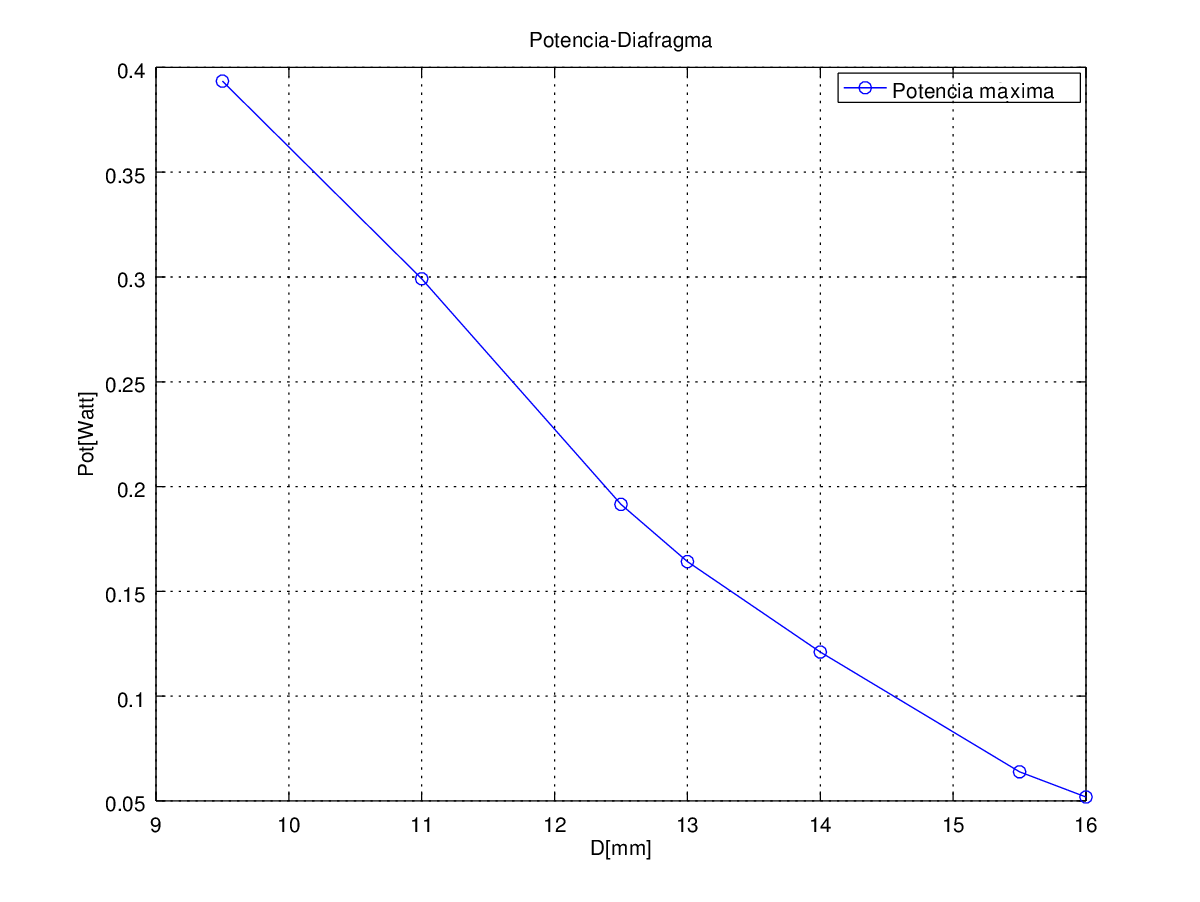
\includegraphics{potmaxDCanal3D.png}
\caption{Potencia extraida por cada diafragma [9,5-11-12,5-13-14-15,5-16]}
\label{fig:potmaxDCanal3D}
\end{figure}

Además, mediante la siguiente gráfica se puede determinar que el volumen
de agua, al permanecer invariable para todos los casos, alcanza una
altura dentro de la cámara, prácticamente constante. No obstante, se ve
algo alterado el máximo valor logrado, ya que la oposición de la salida
de aire, provocada por el diámetro de placa más pequeño hará que parte
del agua no entre. De forma análoga, el caudal de aire que pasa a través
del diafragma, será mayor, cuanto mayor sea el diámetro de la salida de
éste:

\begin{figure}
\centering
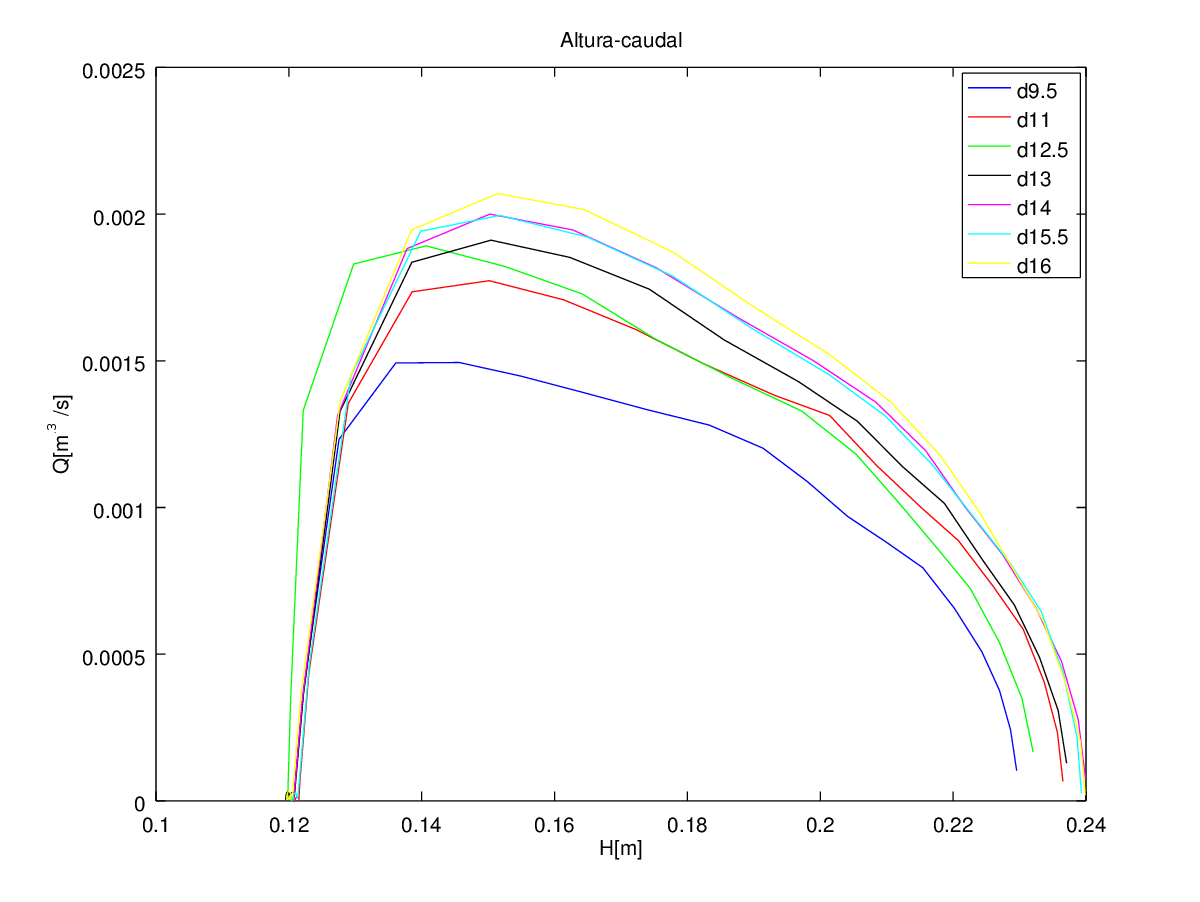
\includegraphics{HQdiaf.png}
\caption[Caudal de aire por la chimenea]{Caudal de aire por la chimenea respecto a la altura de agua dentro de la cámara}
\label{fig:HQdiaf}
\end{figure}
